\section{The Base Configuration}\label{sec:main-result}

In this section we present the base configuration of $19$ straight lines
(Figure~\ref{fig:base-configuration}) and establish its properties that allow us
to apply the iterative step from Proposition~\ref{prop:iterative-step}.

\begin{figure}[ht]
\centering
\resizebox{1.0\textwidth}{!}{% Generated by Visual Arnold
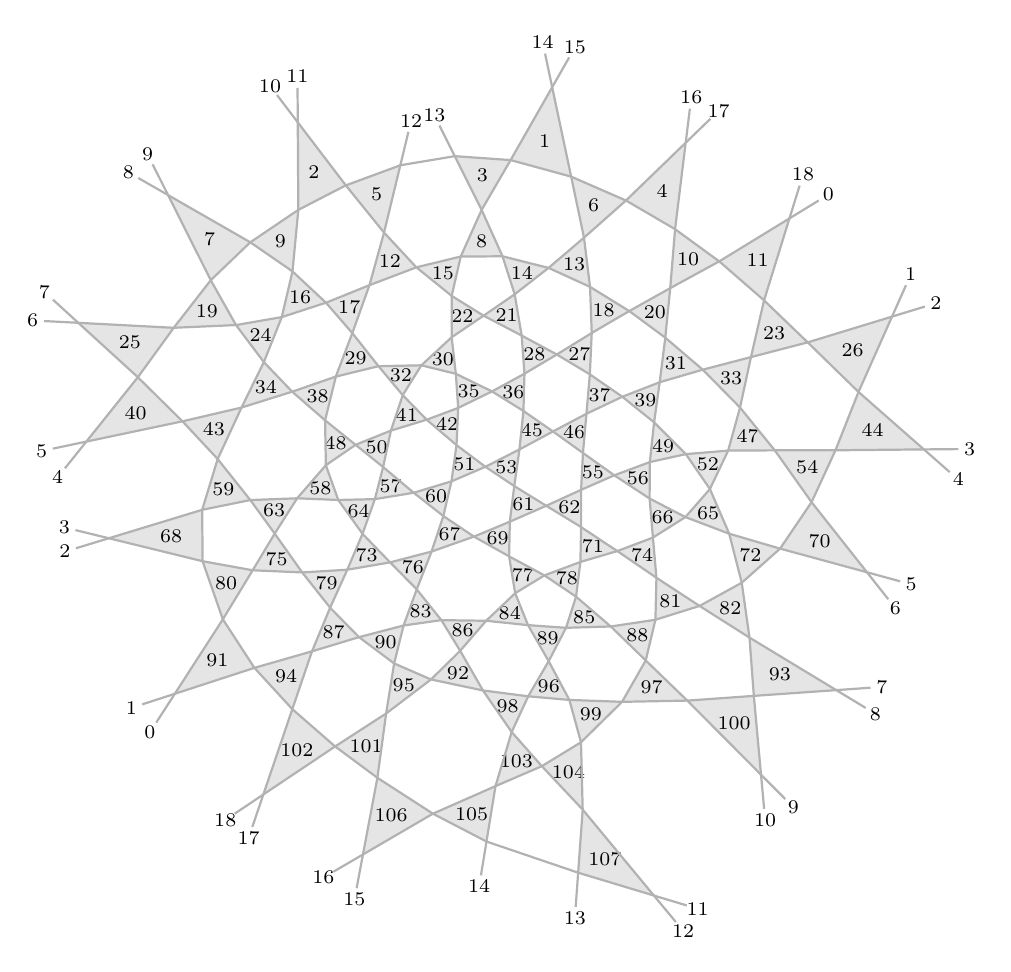
\begin{tikzpicture}[x=\linewidth,y=\linewidth,
  poly/.style={fill=gray!20},
  ext/.style={gray!60,thick},
  lbl/.style={inner sep=0pt,font=\scriptsize},
  plbl/.style={inner sep=0pt,font=\scriptsize}]
\useasboundingbox (0,0) rectangle (1,-0.96007);
\clip (0,0) rectangle (1,-0.96007);
\fill[poly] (0.16215,-0.41229) -- (0.06148,-0.43351) -- (0.11542,-0.36614) -- cycle;
\fill[poly] (0.15299,-0.31434) -- (0.11542,-0.36614) -- (0.05301,-0.30913) -- cycle;
\fill[poly] (0.21820,-0.31148) -- (0.15299,-0.31434) -- (0.19175,-0.26449) -- cycle;
\fill[poly] (0.23319,-0.22480) -- (0.19175,-0.26449) -- (0.14704,-0.17534) -- cycle;
\fill[poly] (0.27736,-0.25527) -- (0.23319,-0.22480) -- (0.28348,-0.19081) -- cycle;
\fill[poly] (0.24738,-0.35028) -- (0.21820,-0.31148) -- (0.26614,-0.30315) -- cycle;
\fill[poly] (0.19901,-0.45180) -- (0.16215,-0.41229) -- (0.22399,-0.39788) -- cycle;
\fill[poly] (0.18319,-0.55880) -- (0.08498,-0.53478) -- (0.18278,-0.50501) -- cycle;
\fill[poly] (0.23749,-0.67052) -- (0.15412,-0.69766) -- (0.20443,-0.61971) -- cycle;
\fill[poly] (0.23566,-0.56832) -- (0.20443,-0.61971) -- (0.18319,-0.55880) -- cycle;
\fill[poly] (0.23320,-0.49475) -- (0.18278,-0.50501) -- (0.19901,-0.45180) -- cycle;
\fill[poly] (0.28757,-0.57057) -- (0.23566,-0.56832) -- (0.25873,-0.52990) -- cycle;
\fill[poly] (0.28222,-0.49292) -- (0.25873,-0.52990) -- (0.23320,-0.49475) -- cycle;
\fill[poly] (0.27705,-0.38127) -- (0.22399,-0.39788) -- (0.24738,-0.35028) -- cycle;
\fill[poly] (0.31244,-0.28807) -- (0.26614,-0.30315) -- (0.27736,-0.25527) -- cycle;
\fill[poly] (0.33322,-0.16518) -- (0.28348,-0.19081) -- (0.28289,-0.09911) -- cycle;
\fill[poly] (0.37324,-0.21465) -- (0.33322,-0.16518) -- (0.39030,-0.14414) -- cycle;
\fill[poly] (0.34003,-0.31988) -- (0.31244,-0.28807) -- (0.35798,-0.26970) -- cycle;
\fill[poly] (0.31149,-0.41126) -- (0.27705,-0.38127) -- (0.32275,-0.36546) -- cycle;
\fill[poly] (0.32530,-0.49468) -- (0.28222,-0.49292) -- (0.31232,-0.45830) -- cycle;
\fill[poly] (0.34346,-0.43690) -- (0.31232,-0.45830) -- (0.31149,-0.41126) -- cycle;
\fill[poly] (0.36746,-0.35456) -- (0.32275,-0.36546) -- (0.34003,-0.31988) -- cycle;
\fill[poly] (0.40711,-0.25101) -- (0.35798,-0.26970) -- (0.37324,-0.21465) -- cycle;
\fill[poly] (0.47547,-0.19086) -- (0.44735,-0.13457) -- (0.50581,-0.13868) -- cycle;
\fill[poly] (0.44408,-0.28091) -- (0.40711,-0.25101) -- (0.45360,-0.23971) -- cycle;
\fill[poly] (0.49736,-0.23945) -- (0.45360,-0.23971) -- (0.47547,-0.19086) -- cycle;
\fill[poly] (0.56924,-0.15602) -- (0.50581,-0.13868) -- (0.54936,-0.06237) -- cycle;
\fill[poly] (0.58269,-0.21995) -- (0.56924,-0.15602) -- (0.62665,-0.18102) -- cycle;
\fill[poly] (0.51008,-0.27927) -- (0.49736,-0.23945) -- (0.54557,-0.25161) -- cycle;
\fill[poly] (0.44407,-0.32427) -- (0.44408,-0.28091) -- (0.47752,-0.30165) -- cycle;
\fill[poly] (0.39280,-0.38488) -- (0.36746,-0.35456) -- (0.41234,-0.35364) -- cycle;
\fill[poly] (0.37227,-0.46017) -- (0.34346,-0.43690) -- (0.38047,-0.42201) -- cycle;
\fill[poly] (0.35071,-0.53014) -- (0.32530,-0.49468) -- (0.36365,-0.49381) -- cycle;
\fill[poly] (0.31678,-0.60751) -- (0.28757,-0.57057) -- (0.33477,-0.56772) -- cycle;
\fill[poly] (0.27718,-0.71377) -- (0.23749,-0.67052) -- (0.29781,-0.65320) -- cycle;
\fill[poly] (0.34705,-0.63835) -- (0.29781,-0.65320) -- (0.31678,-0.60751) -- cycle;
\fill[poly] (0.37964,-0.56004) -- (0.33477,-0.56772) -- (0.35071,-0.53014) -- cycle;
\fill[poly] (0.40435,-0.48712) -- (0.36365,-0.49381) -- (0.37227,-0.46017) -- cycle;
\fill[poly] (0.41791,-0.41061) -- (0.38047,-0.42201) -- (0.39280,-0.38488) -- cycle;
\fill[poly] (0.44844,-0.36252) -- (0.41234,-0.35364) -- (0.44407,-0.32427) -- cycle;
\fill[poly] (0.44914,-0.43720) -- (0.41791,-0.41061) -- (0.45092,-0.39826) -- cycle;
\fill[poly] (0.43536,-0.51150) -- (0.40435,-0.48712) -- (0.44388,-0.47519) -- cycle;
\fill[poly] (0.40749,-0.58826) -- (0.37964,-0.56004) -- (0.42302,-0.54871) -- cycle;
\fill[poly] (0.38384,-0.66590) -- (0.34705,-0.63835) -- (0.39370,-0.62618) -- cycle;
\fill[poly] (0.43332,-0.62055) -- (0.39370,-0.62618) -- (0.40749,-0.58826) -- cycle;
\fill[poly] (0.46742,-0.53305) -- (0.42302,-0.54871) -- (0.43536,-0.51150) -- cycle;
\fill[poly] (0.47945,-0.45992) -- (0.44388,-0.47519) -- (0.44914,-0.43720) -- cycle;
\fill[poly] (0.48634,-0.38096) -- (0.45092,-0.39826) -- (0.44844,-0.36252) -- cycle;
\fill[poly] (0.51742,-0.32248) -- (0.47752,-0.30165) -- (0.51008,-0.27927) -- cycle;
\fill[poly] (0.51926,-0.40148) -- (0.48634,-0.38096) -- (0.52032,-0.36248) -- cycle;
\fill[poly] (0.50966,-0.48010) -- (0.47945,-0.45992) -- (0.51508,-0.44174) -- cycle;
\fill[poly] (0.50426,-0.55374) -- (0.46742,-0.53305) -- (0.50498,-0.51742) -- cycle;
\fill[poly] (0.54314,-0.50075) -- (0.50498,-0.51742) -- (0.50966,-0.48010) -- cycle;
\fill[poly] (0.55019,-0.42291) -- (0.51508,-0.44174) -- (0.51926,-0.40148) -- cycle;
\fill[poly] (0.55421,-0.34231) -- (0.52032,-0.36248) -- (0.51742,-0.32248) -- cycle;
\fill[poly] (0.58901,-0.27147) -- (0.54557,-0.25161) -- (0.58269,-0.21995) -- cycle;
\fill[poly] (0.58882,-0.36312) -- (0.55421,-0.34231) -- (0.59077,-0.31980) -- cycle;
\fill[poly] (0.58160,-0.44544) -- (0.55019,-0.42291) -- (0.58523,-0.40439) -- cycle;
\fill[poly] (0.57966,-0.52309) -- (0.54314,-0.50075) -- (0.57966,-0.48409) -- cycle;
\fill[poly] (0.61441,-0.46884) -- (0.57966,-0.48409) -- (0.58160,-0.44544) -- cycle;
\fill[poly] (0.62285,-0.38657) -- (0.58523,-0.40439) -- (0.58882,-0.36312) -- cycle;
\fill[poly] (0.63009,-0.29680) -- (0.59077,-0.31980) -- (0.58901,-0.27147) -- cycle;
\fill[poly] (0.67807,-0.21105) -- (0.62665,-0.18102) -- (0.68920,-0.12050) -- cycle;
\fill[poly] (0.66783,-0.32471) -- (0.63009,-0.29680) -- (0.67299,-0.27281) -- cycle;
\fill[poly] (0.65609,-0.41339) -- (0.62285,-0.38657) -- (0.66197,-0.37135) -- cycle;
\fill[poly] (0.65138,-0.49318) -- (0.61441,-0.46884) -- (0.65163,-0.45498) -- cycle;
\fill[poly] (0.68937,-0.44665) -- (0.65163,-0.45498) -- (0.65609,-0.41339) -- cycle;
\fill[poly] (0.70706,-0.35822) -- (0.66197,-0.37135) -- (0.66783,-0.32471) -- cycle;
\fill[poly] (0.72433,-0.24476) -- (0.67299,-0.27281) -- (0.67807,-0.21105) -- cycle;
\fill[poly] (0.77127,-0.28558) -- (0.72433,-0.24476) -- (0.79787,-0.19978) -- cycle;
\fill[poly] (0.74611,-0.39785) -- (0.70706,-0.35822) -- (0.75756,-0.34503) -- cycle;
\fill[poly] (0.71457,-0.48322) -- (0.68937,-0.44665) -- (0.73368,-0.44296) -- cycle;
\fill[poly] (0.65488,-0.53409) -- (0.65138,-0.49318) -- (0.68891,-0.51260) -- cycle;
\fill[poly] (0.57893,-0.55959) -- (0.57966,-0.52309) -- (0.61755,-0.54821) -- cycle;
\fill[poly] (0.51057,-0.59234) -- (0.50426,-0.55374) -- (0.54126,-0.57369) -- cycle;
\fill[poly] (0.45299,-0.65264) -- (0.43332,-0.62055) -- (0.48020,-0.62120) -- cycle;
\fill[poly] (0.37544,-0.71831) -- (0.38384,-0.66590) -- (0.42242,-0.68266) -- cycle;
\fill[poly] (0.24684,-0.80315) -- (0.27718,-0.71377) -- (0.32203,-0.75283) -- cycle;
\fill[poly] (0.36629,-0.78567) -- (0.32203,-0.75283) -- (0.37544,-0.71831) -- cycle;
\fill[poly] (0.47686,-0.69418) -- (0.42242,-0.68266) -- (0.45299,-0.65264) -- cycle;
\fill[poly] (0.52406,-0.62576) -- (0.48020,-0.62120) -- (0.51057,-0.59234) -- cycle;
\fill[poly] (0.57437,-0.59595) -- (0.54126,-0.57369) -- (0.57893,-0.55959) -- cycle;
\fill[poly] (0.54570,-0.66353) -- (0.52406,-0.62576) -- (0.56386,-0.62857) -- cycle;
\fill[poly] (0.50693,-0.73770) -- (0.47686,-0.69418) -- (0.52424,-0.70031) -- cycle;
\fill[poly] (0.56737,-0.70410) -- (0.52424,-0.70031) -- (0.54570,-0.66353) -- cycle;
\fill[poly] (0.61072,-0.62718) -- (0.56386,-0.62857) -- (0.57437,-0.59595) -- cycle;
\fill[poly] (0.65856,-0.57614) -- (0.61755,-0.54821) -- (0.65488,-0.53409) -- cycle;
\fill[poly] (0.64734,-0.66274) -- (0.61072,-0.62718) -- (0.65749,-0.62017) -- cycle;
\fill[poly] (0.57955,-0.74846) -- (0.56737,-0.70410) -- (0.62258,-0.70610) -- cycle;
\fill[poly] (0.49000,-0.79440) -- (0.50693,-0.73770) -- (0.53853,-0.77348) -- cycle;
\fill[poly] (0.35116,-0.86601) -- (0.36629,-0.78567) -- (0.42445,-0.82325) -- cycle;
\fill[poly] (0.48054,-0.85241) -- (0.42445,-0.82325) -- (0.49000,-0.79440) -- cycle;
\fill[poly] (0.58131,-0.81899) -- (0.53853,-0.77348) -- (0.57955,-0.74846) -- cycle;
\fill[poly] (0.65590,-0.90899) -- (0.57656,-0.88504) -- (0.58131,-0.81899) -- cycle;
\fill[poly] (0.69088,-0.70482) -- (0.62258,-0.70610) -- (0.64734,-0.66274) -- cycle;
\fill[poly] (0.70372,-0.60567) -- (0.65749,-0.62017) -- (0.65856,-0.57614) -- cycle;
\fill[poly] (0.73477,-0.53001) -- (0.68891,-0.51260) -- (0.71457,-0.48322) -- cycle;
\fill[poly] (0.75601,-0.63882) -- (0.70372,-0.60567) -- (0.74791,-0.58136) -- cycle;
\fill[poly] (0.76810,-0.78245) -- (0.69088,-0.70482) -- (0.76058,-0.69987) -- cycle;
\fill[poly] (0.84689,-0.69383) -- (0.76058,-0.69987) -- (0.75601,-0.63882) -- cycle;
\fill[poly] (0.78807,-0.54563) -- (0.74791,-0.58136) -- (0.73477,-0.53001) -- cycle;
\fill[poly] (0.78250,-0.44271) -- (0.73368,-0.44296) -- (0.74611,-0.39785) -- cycle;
\fill[poly] (0.87908,-0.57041) -- (0.78807,-0.54563) -- (0.82103,-0.49697) -- cycle;
\fill[poly] (0.84607,-0.44262) -- (0.82103,-0.49697) -- (0.78250,-0.44271) -- cycle;
\fill[poly] (0.81697,-0.32961) -- (0.75756,-0.34503) -- (0.77127,-0.28558) -- cycle;
\fill[poly] (0.93870,-0.44173) -- (0.84607,-0.44262) -- (0.87020,-0.38154) -- cycle;
\fill[poly] (0.90532,-0.30262) -- (0.87020,-0.38154) -- (0.81697,-0.32961) -- cycle;
\node[plbl] at (0.11302,-0.40398) {40};
\node[plbl] at (0.10714,-0.32987) {25};
\node[plbl] at (0.18764,-0.29677) {19};
\node[plbl] at (0.19066,-0.22154) {7};
\node[plbl] at (0.26468,-0.22363) {9};
\node[plbl] at (0.24391,-0.32164) {24};
\node[plbl] at (0.19505,-0.42066) {43};
\node[plbl] at (0.15032,-0.53286) {68};
\node[plbl] at (0.19868,-0.66263) {91};
\node[plbl] at (0.20776,-0.58228) {80};
\node[plbl] at (0.20500,-0.48385) {59};
\node[plbl] at (0.26066,-0.55626) {75};
\node[plbl] at (0.25805,-0.50585) {63};
\node[plbl] at (0.24947,-0.37648) {34};
\node[plbl] at (0.28531,-0.28216) {16};
\node[plbl] at (0.29986,-0.15170) {2};
\node[plbl] at (0.36559,-0.17466) {5};
\node[plbl] at (0.33682,-0.29255) {17};
\node[plbl] at (0.30376,-0.38600) {38};
\node[plbl] at (0.30661,-0.48197) {58};
\node[plbl] at (0.32242,-0.43549) {48};
\node[plbl] at (0.34341,-0.34664) {29};
\node[plbl] at (0.37944,-0.24512) {12};
\node[plbl] at (0.47621,-0.15470) {3};
\node[plbl] at (0.43493,-0.25721) {15};
\node[plbl] at (0.47548,-0.22334) {8};
\node[plbl] at (0.54147,-0.11902) {1};
\node[plbl] at (0.59286,-0.18566) {6};
\node[plbl] at (0.51767,-0.25677) {14};
\node[plbl] at (0.45523,-0.30228) {22};
\node[plbl] at (0.39087,-0.36436) {32};
\node[plbl] at (0.36540,-0.43969) {50};
\node[plbl] at (0.34656,-0.50621) {64};
\node[plbl] at (0.31304,-0.58193) {79};
\node[plbl] at (0.27083,-0.67916) {94};
\node[plbl] at (0.32055,-0.63302) {87};
\node[plbl] at (0.35504,-0.55264) {73};
\node[plbl] at (0.38009,-0.48037) {57};
\node[plbl] at (0.39706,-0.40583) {41};
\node[plbl] at (0.43495,-0.34681) {30};
\node[plbl] at (0.43933,-0.41536) {42};
\node[plbl] at (0.42786,-0.49127) {60};
\node[plbl] at (0.40338,-0.56567) {76};
\node[plbl] at (0.37487,-0.64348) {90};
\node[plbl] at (0.41150,-0.61167) {83};
\node[plbl] at (0.44193,-0.53109) {67};
\node[plbl] at (0.45749,-0.45743) {51};
\node[plbl] at (0.46190,-0.38058) {35};
\node[plbl] at (0.50167,-0.30113) {21};
\node[plbl] at (0.50864,-0.38164) {36};
\node[plbl] at (0.50140,-0.46059) {53};
\node[plbl] at (0.49222,-0.53474) {69};
\node[plbl] at (0.51926,-0.49942) {61};
\node[plbl] at (0.52818,-0.42205) {45};
\node[plbl] at (0.53065,-0.34242) {28};
\node[plbl] at (0.57242,-0.24768) {13};
\node[plbl] at (0.57793,-0.34174) {27};
\node[plbl] at (0.57234,-0.42425) {46};
\node[plbl] at (0.56749,-0.50264) {62};
\node[plbl] at (0.59189,-0.46612) {55};
\node[plbl] at (0.59897,-0.38469) {37};
\node[plbl] at (0.60329,-0.29602) {18};
\node[plbl] at (0.66464,-0.17086) {4};
\node[plbl] at (0.65697,-0.29811) {20};
\node[plbl] at (0.64697,-0.39043) {39};
\node[plbl] at (0.63914,-0.47233) {56};
\node[plbl] at (0.66570,-0.43834) {49};
\node[plbl] at (0.67896,-0.35143) {31};
\node[plbl] at (0.69180,-0.24287) {10};
\node[plbl] at (0.76449,-0.24337) {11};
\node[plbl] at (0.73691,-0.36703) {33};
\node[plbl] at (0.71254,-0.45761) {52};
\node[plbl] at (0.66506,-0.51329) {66};
\node[plbl] at (0.59205,-0.54363) {71};
\node[plbl] at (0.51870,-0.57326) {77};
\node[plbl] at (0.45550,-0.63146) {86};
\node[plbl] at (0.39390,-0.68896) {95};
\node[plbl] at (0.28201,-0.75659) {102};
\node[plbl] at (0.35458,-0.75227) {101};
\node[plbl] at (0.45075,-0.67649) {92};
\node[plbl] at (0.50494,-0.61310) {84};
\node[plbl] at (0.56486,-0.57641) {78};
\node[plbl] at (0.54454,-0.63929) {89};
\node[plbl] at (0.50267,-0.71073) {98};
\node[plbl] at (0.54577,-0.68931) {96};
\node[plbl] at (0.58298,-0.61723) {85};
\node[plbl] at (0.64366,-0.55282) {74};
\node[plbl] at (0.63851,-0.63669) {88};
\node[plbl] at (0.58983,-0.71955) {99};
\node[plbl] at (0.51182,-0.76853) {103};
\node[plbl] at (0.38064,-0.82498) {106};
\node[plbl] at (0.46500,-0.82335) {105};
\node[plbl] at (0.56646,-0.78031) {104};
\node[plbl] at (0.60459,-0.87101) {107};
\node[plbl] at (0.65360,-0.69122) {97};
\node[plbl] at (0.67325,-0.60066) {81};
\node[plbl] at (0.71275,-0.50861) {65};
\node[plbl] at (0.73588,-0.60861) {82};
\node[plbl] at (0.73985,-0.72905) {100};
\node[plbl] at (0.78783,-0.67751) {93};
\node[plbl] at (0.75692,-0.55233) {72};
\node[plbl] at (0.75410,-0.42784) {47};
\node[plbl] at (0.82939,-0.53767) {70};
\node[plbl] at (0.81654,-0.46077) {54};
\node[plbl] at (0.78193,-0.32008) {23};
\node[plbl] at (0.88499,-0.42196) {44};
\node[plbl] at (0.86416,-0.33792) {26};
\draw[ext] (0.13462,-0.72788) -- (0.15412,-0.69766) -- (0.20443,-0.61971) -- (0.23566,-0.56832) -- (0.25873,-0.52990) -- (0.28222,-0.49292) -- (0.31232,-0.45830) -- (0.34346,-0.43690) -- (0.38047,-0.42201) -- (0.41791,-0.41061) -- (0.45092,-0.39826) -- (0.48634,-0.38096) -- (0.52032,-0.36248) -- (0.55421,-0.34231) -- (0.59077,-0.31980) -- (0.63009,-0.29680) -- (0.67299,-0.27281) -- (0.72433,-0.24476) -- (0.79787,-0.19978) -- (0.82855,-0.18101);
\node[lbl] at (0.12811,-0.73796) {0};
\node[lbl] at (0.83879,-0.17475) {0};
\draw[ext] (0.11992,-0.70879) -- (0.15412,-0.69766) -- (0.23749,-0.67052) -- (0.29781,-0.65320) -- (0.34705,-0.63835) -- (0.39370,-0.62618) -- (0.43332,-0.62055) -- (0.48020,-0.62120) -- (0.52406,-0.62576) -- (0.56386,-0.62857) -- (0.61072,-0.62718) -- (0.65749,-0.62017) -- (0.70372,-0.60567) -- (0.74791,-0.58136) -- (0.78807,-0.54563) -- (0.82103,-0.49697) -- (0.84607,-0.44262) -- (0.87020,-0.38154) -- (0.90532,-0.30262) -- (0.91994,-0.26976);
\node[lbl] at (0.10851,-0.71250) {1};
\node[lbl] at (0.92482,-0.25879) {1};
\draw[ext] (0.05058,-0.54525) -- (0.08498,-0.53478) -- (0.18278,-0.50501) -- (0.23320,-0.49475) -- (0.28222,-0.49292) -- (0.32530,-0.49468) -- (0.36365,-0.49381) -- (0.40435,-0.48712) -- (0.44388,-0.47519) -- (0.47945,-0.45992) -- (0.51508,-0.44174) -- (0.55019,-0.42291) -- (0.58523,-0.40439) -- (0.62285,-0.38657) -- (0.66197,-0.37135) -- (0.70706,-0.35822) -- (0.75756,-0.34503) -- (0.81697,-0.32961) -- (0.90532,-0.30262) -- (0.93971,-0.29211);
\node[lbl] at (0.03910,-0.54875) {2};
\node[lbl] at (0.95119,-0.28860) {2};
\draw[ext] (0.05005,-0.52623) -- (0.08498,-0.53478) -- (0.18319,-0.55880) -- (0.23566,-0.56832) -- (0.28757,-0.57057) -- (0.33477,-0.56772) -- (0.37964,-0.56004) -- (0.42302,-0.54871) -- (0.46742,-0.53305) -- (0.50498,-0.51742) -- (0.54314,-0.50075) -- (0.57966,-0.48409) -- (0.61441,-0.46884) -- (0.65163,-0.45498) -- (0.68937,-0.44665) -- (0.73368,-0.44296) -- (0.78250,-0.44271) -- (0.84607,-0.44262) -- (0.93870,-0.44173) -- (0.97467,-0.44139);
\node[lbl] at (0.03839,-0.52338) {3};
\node[lbl] at (0.98666,-0.44127) {3};
\draw[ext] (0.03899,-0.46158) -- (0.06148,-0.43351) -- (0.11542,-0.36614) -- (0.15299,-0.31434) -- (0.19175,-0.26449) -- (0.23319,-0.22480) -- (0.28348,-0.19081) -- (0.33322,-0.16518) -- (0.39030,-0.14414) -- (0.44735,-0.13457) -- (0.50581,-0.13868) -- (0.56924,-0.15602) -- (0.62665,-0.18102) -- (0.67807,-0.21105) -- (0.72433,-0.24476) -- (0.77127,-0.28558) -- (0.81697,-0.32961) -- (0.87020,-0.38154) -- (0.93870,-0.44173) -- (0.96572,-0.46547);
\node[lbl] at (0.03149,-0.47095) {4};
\node[lbl] at (0.97473,-0.47339) {4};
\draw[ext] (0.02628,-0.44092) -- (0.06148,-0.43351) -- (0.16215,-0.41229) -- (0.22399,-0.39788) -- (0.27705,-0.38127) -- (0.32275,-0.36546) -- (0.36746,-0.35456) -- (0.41234,-0.35364) -- (0.44844,-0.36252) -- (0.48634,-0.38096) -- (0.51926,-0.40148) -- (0.55019,-0.42291) -- (0.58160,-0.44544) -- (0.61441,-0.46884) -- (0.65138,-0.49318) -- (0.68891,-0.51260) -- (0.73477,-0.53001) -- (0.78807,-0.54563) -- (0.87908,-0.57041) -- (0.91378,-0.57986);
\node[lbl] at (0.01454,-0.44340) {5};
\node[lbl] at (0.92536,-0.58302) {5};
\draw[ext] (0.01710,-0.30726) -- (0.05301,-0.30913) -- (0.15299,-0.31434) -- (0.21820,-0.31148) -- (0.26614,-0.30315) -- (0.31244,-0.28807) -- (0.35798,-0.26970) -- (0.40711,-0.25101) -- (0.45360,-0.23971) -- (0.49736,-0.23945) -- (0.54557,-0.25161) -- (0.58901,-0.27147) -- (0.63009,-0.29680) -- (0.66783,-0.32471) -- (0.70706,-0.35822) -- (0.74611,-0.39785) -- (0.78250,-0.44271) -- (0.82103,-0.49697) -- (0.87908,-0.57041) -- (0.90138,-0.59863);
\node[lbl] at (0.00511,-0.30663) {6};
\node[lbl] at (0.90882,-0.60805) {6};
\draw[ext] (0.02646,-0.28487) -- (0.05301,-0.30913) -- (0.11542,-0.36614) -- (0.16215,-0.41229) -- (0.19901,-0.45180) -- (0.23320,-0.49475) -- (0.25873,-0.52990) -- (0.28757,-0.57057) -- (0.31678,-0.60751) -- (0.34705,-0.63835) -- (0.38384,-0.66590) -- (0.42242,-0.68266) -- (0.47686,-0.69418) -- (0.52424,-0.70031) -- (0.56737,-0.70410) -- (0.62258,-0.70610) -- (0.69088,-0.70482) -- (0.76058,-0.69987) -- (0.84689,-0.69383) -- (0.88277,-0.69132);
\node[lbl] at (0.01760,-0.27678) {7};
\node[lbl] at (0.89474,-0.69048) {7};
\draw[ext] (0.11585,-0.15743) -- (0.14704,-0.17534) -- (0.23319,-0.22480) -- (0.27736,-0.25527) -- (0.31244,-0.28807) -- (0.34003,-0.31988) -- (0.36746,-0.35456) -- (0.39280,-0.38488) -- (0.41791,-0.41061) -- (0.44914,-0.43720) -- (0.47945,-0.45992) -- (0.50966,-0.48010) -- (0.54314,-0.50075) -- (0.57966,-0.52309) -- (0.61755,-0.54821) -- (0.65856,-0.57614) -- (0.70372,-0.60567) -- (0.75601,-0.63882) -- (0.84689,-0.69383) -- (0.87766,-0.71246);
\node[lbl] at (0.10544,-0.15146) {8};
\node[lbl] at (0.88793,-0.71867) {8};
\draw[ext] (0.13091,-0.14319) -- (0.14704,-0.17534) -- (0.19175,-0.26449) -- (0.21820,-0.31148) -- (0.24738,-0.35028) -- (0.27705,-0.38127) -- (0.31149,-0.41126) -- (0.34346,-0.43690) -- (0.37227,-0.46017) -- (0.40435,-0.48712) -- (0.43536,-0.51150) -- (0.46742,-0.53305) -- (0.50426,-0.55374) -- (0.54126,-0.57369) -- (0.57437,-0.59595) -- (0.61072,-0.62718) -- (0.64734,-0.66274) -- (0.69088,-0.70482) -- (0.76810,-0.78245) -- (0.79347,-0.80795);
\node[lbl] at (0.12554,-0.13246) {9};
\node[lbl] at (0.80193,-0.81646) {9};
\draw[ext] (0.26109,-0.07050) -- (0.28289,-0.09911) -- (0.33322,-0.16518) -- (0.37324,-0.21465) -- (0.40711,-0.25101) -- (0.44408,-0.28091) -- (0.47752,-0.30165) -- (0.51742,-0.32248) -- (0.55421,-0.34231) -- (0.58882,-0.36312) -- (0.62285,-0.38657) -- (0.65609,-0.41339) -- (0.68937,-0.44665) -- (0.71457,-0.48322) -- (0.73477,-0.53001) -- (0.74791,-0.58136) -- (0.75601,-0.63882) -- (0.76058,-0.69987) -- (0.76810,-0.78245) -- (0.77136,-0.81827);
\node[lbl] at (0.25382,-0.06095) {10};
\node[lbl] at (0.77245,-0.83022) {10};
\draw[ext] (0.28265,-0.06314) -- (0.28289,-0.09911) -- (0.28348,-0.19081) -- (0.27736,-0.25527) -- (0.26614,-0.30315) -- (0.24738,-0.35028) -- (0.22399,-0.39788) -- (0.19901,-0.45180) -- (0.18278,-0.50501) -- (0.18319,-0.55880) -- (0.20443,-0.61971) -- (0.23749,-0.67052) -- (0.27718,-0.71377) -- (0.32203,-0.75283) -- (0.36629,-0.78567) -- (0.42445,-0.82325) -- (0.48054,-0.85241) -- (0.57656,-0.88504) -- (0.65590,-0.90899) -- (0.69034,-0.91938);
\node[lbl] at (0.28257,-0.05114) {11};
\node[lbl] at (0.70182,-0.92285) {11};
\draw[ext] (0.39876,-0.10918) -- (0.39030,-0.14414) -- (0.37324,-0.21465) -- (0.35798,-0.26970) -- (0.34003,-0.31988) -- (0.32275,-0.36546) -- (0.31149,-0.41126) -- (0.31232,-0.45830) -- (0.32530,-0.49468) -- (0.35071,-0.53014) -- (0.37964,-0.56004) -- (0.40749,-0.58826) -- (0.43332,-0.62055) -- (0.45299,-0.65264) -- (0.47686,-0.69418) -- (0.50693,-0.73770) -- (0.53853,-0.77348) -- (0.58131,-0.81899) -- (0.65590,-0.90899) -- (0.67886,-0.93668);
\node[lbl] at (0.40159,-0.09752) {12};
\node[lbl] at (0.68651,-0.94592) {12};
\draw[ext] (0.43128,-0.10240) -- (0.44735,-0.13457) -- (0.47547,-0.19086) -- (0.49736,-0.23945) -- (0.51008,-0.27927) -- (0.51742,-0.32248) -- (0.52032,-0.36248) -- (0.51926,-0.40148) -- (0.51508,-0.44174) -- (0.50966,-0.48010) -- (0.50498,-0.51742) -- (0.50426,-0.55374) -- (0.51057,-0.59234) -- (0.52406,-0.62576) -- (0.54570,-0.66353) -- (0.56737,-0.70410) -- (0.57955,-0.74846) -- (0.58131,-0.81899) -- (0.57656,-0.88504) -- (0.57398,-0.92091);
\node[lbl] at (0.42592,-0.09166) {13};
\node[lbl] at (0.57311,-0.93288) {13};
\draw[ext] (0.54189,-0.02718) -- (0.54936,-0.06237) -- (0.56924,-0.15602) -- (0.58269,-0.21995) -- (0.58901,-0.27147) -- (0.59077,-0.31980) -- (0.58882,-0.36312) -- (0.58523,-0.40439) -- (0.58160,-0.44544) -- (0.57966,-0.48409) -- (0.57966,-0.52309) -- (0.57893,-0.55959) -- (0.57437,-0.59595) -- (0.56386,-0.62857) -- (0.54570,-0.66353) -- (0.52424,-0.70031) -- (0.50693,-0.73770) -- (0.49000,-0.79440) -- (0.48054,-0.85241) -- (0.47475,-0.88790);
\node[lbl] at (0.53939,-0.01545) {14};
\node[lbl] at (0.47282,-0.89975) {14};
\draw[ext] (0.56718,-0.03113) -- (0.54936,-0.06237) -- (0.50581,-0.13868) -- (0.47547,-0.19086) -- (0.45360,-0.23971) -- (0.44408,-0.28091) -- (0.44407,-0.32427) -- (0.44844,-0.36252) -- (0.45092,-0.39826) -- (0.44914,-0.43720) -- (0.44388,-0.47519) -- (0.43536,-0.51150) -- (0.42302,-0.54871) -- (0.40749,-0.58826) -- (0.39370,-0.62618) -- (0.38384,-0.66590) -- (0.37544,-0.71831) -- (0.36629,-0.78567) -- (0.35116,-0.86601) -- (0.34451,-0.90135);
\node[lbl] at (0.57313,-0.02070) {15};
\node[lbl] at (0.34229,-0.91315) {15};
\draw[ext] (0.69359,-0.08480) -- (0.68920,-0.12050) -- (0.67807,-0.21105) -- (0.67299,-0.27281) -- (0.66783,-0.32471) -- (0.66197,-0.37135) -- (0.65609,-0.41339) -- (0.65163,-0.45498) -- (0.65138,-0.49318) -- (0.65488,-0.53409) -- (0.65856,-0.57614) -- (0.65749,-0.62017) -- (0.64734,-0.66274) -- (0.62258,-0.70610) -- (0.57955,-0.74846) -- (0.53853,-0.77348) -- (0.49000,-0.79440) -- (0.42445,-0.82325) -- (0.35116,-0.86601) -- (0.32010,-0.88413);
\node[lbl] at (0.69506,-0.07289) {16};
\node[lbl] at (0.30973,-0.89018) {16};
\draw[ext] (0.71505,-0.09549) -- (0.68920,-0.12050) -- (0.62665,-0.18102) -- (0.58269,-0.21995) -- (0.54557,-0.25161) -- (0.51008,-0.27927) -- (0.47752,-0.30165) -- (0.44407,-0.32427) -- (0.41234,-0.35364) -- (0.39280,-0.38488) -- (0.38047,-0.42201) -- (0.37227,-0.46017) -- (0.36365,-0.49381) -- (0.35071,-0.53014) -- (0.33477,-0.56772) -- (0.31678,-0.60751) -- (0.29781,-0.65320) -- (0.27718,-0.71377) -- (0.24684,-0.80315) -- (0.23528,-0.83721);
\node[lbl] at (0.72368,-0.08714) {17};
\node[lbl] at (0.23142,-0.84857) {17};
\draw[ext] (0.80852,-0.16543) -- (0.79787,-0.19978) -- (0.77127,-0.28558) -- (0.75756,-0.34503) -- (0.74611,-0.39785) -- (0.73368,-0.44296) -- (0.71457,-0.48322) -- (0.68891,-0.51260) -- (0.65488,-0.53409) -- (0.61755,-0.54821) -- (0.57893,-0.55959) -- (0.54126,-0.57369) -- (0.51057,-0.59234) -- (0.48020,-0.62120) -- (0.45299,-0.65264) -- (0.42242,-0.68266) -- (0.37544,-0.71831) -- (0.32203,-0.75283) -- (0.24684,-0.80315) -- (0.21695,-0.82316);
\node[lbl] at (0.81208,-0.15396) {18};
\node[lbl] at (0.20697,-0.82983) {18};
\end{tikzpicture}
}
\caption{Pseudoline diagram of the base configuration with all $107$
bounded triangles numbered. Lines are labeled $0,1,\dots,18$.}
\label{fig:pseudolines}
\end{figure}

The base configuration is the normalized family of straight lines
\begin{equation}\label{eq:seed19-normalized-family}
  Y_0:\ y=0,
  \qquad
  L_i:\ y=m_i(x-a_i),
  \qquad i=1,\dots,18,
\end{equation}
where $a_8=-\eps$, $a_{15}=+\eps$, and the remaining $a_i$ values are
$\pm\tan(k\pi/18)$, $k=1,\dots,8$. The slopes $m_i$ and the parameter $\eps$
may vary in the following range:
\providecommand{\SeedNineteenEpsLower}{10^{-12}}
\providecommand{\SeedNineteenEpsUpper}{10^{-4}}
\providecommand{\SeedNineteenDeltaM}{10^{-4}}
\refstepcounter{equation}\label{eq:seed19-parameter-box}
\[
  \eps \in \left(0,\SeedNineteenEpsUpper\right),
  \qquad
  m_i \in \left[m_i^\ast-\delta_m,m_i^\ast+\delta_m\right],
  \qquad
  \delta_m = \SeedNineteenDeltaM.
  \tag{\theequation}
\]
The exact values of slope centers $m_i^\ast$ and $x$-intercepts $a_i$ are:
\begingroup
\[
\renewcommand{\arraystretch}{1.1}
\begin{array}{ll@{\qquad}ll}
 m_{1}^\ast = -0.18006, & a_{1} = -\tan(8\pi/18) & m_{10}^\ast = -23.07892, & a_{10} = +\tan(3\pi/18) \\
 m_{2}^\ast = -0.25231, & a_{2} = -\tan(4\pi/18) & m_{11}^\ast = 4.39005, & a_{11} = -\tan(7\pi/18) \\
 m_{3}^\ast = -0.32584, & a_{3} = -\tan(6\pi/18) & m_{12}^\ast = 2.90204, & a_{12} = -\tan(3\pi/18) \\
 m_{4}^\ast = -1.74521, & a_{4} = +\tan(7\pi/18) & m_{13}^\ast = 1.31845, & a_{13} = +\tan(2\pi/18) \\
 m_{5}^\ast = -2.17941, & a_{5} = +\tan(1\pi/18) & m_{14}^\ast = 0.90192, & a_{14} = +\tan(4\pi/18) \\
 m_{6}^\ast = -2.79557, & a_{6} = +\tan(5\pi/18) & m_{15}^\ast = 0.84501, & a_{15} = +\eps \\
 m_{7}^\ast = -4.59586, & a_{7} = -\tan(5\pi/18) & m_{16}^\ast = 0.64068, & a_{16} = +\tan(6\pi/18) \\
 m_{8}^\ast = -5.67203, & a_{8} = -\eps & m_{17}^\ast = 0.44393, & a_{17} = -\tan(1\pi/18) \\
 m_{9}^\ast = -7.39905, & a_{9} = -\tan(2\pi/18) & m_{18}^\ast = 0.15548, & a_{18} = +\tan(8\pi/18) \\
\end{array}
\]
\endgroup


The corresponding $\mathrm{O}$-matrix is listed in \eqref{eq:seed19-omatrix},
and Figure~\ref{fig:pseudolines} shows the associated pseudoline diagram.

\refstepcounter{equation}
\begingroup
\noindent\hfill
\begin{minipage}[c]{0.72\linewidth}
\footnotesize
\input{generated/seed19_omatrix}
\end{minipage}%
\hfill(\theequation)\label{eq:seed19-omatrix}
\endgroup

\begin{theorem}[Straight-line base configuration at $n=19$]\label{thm:main-seed}
For every choice of parameters in \eqref{eq:seed19-parameter-box},
the normalized family
\eqref{eq:seed19-normalized-family} is a simple affine arrangement of $19$
straight lines satisfying:
\begin{enumerate}[label=(\arabic*)]
\item $Y_0$ is the line $y=0$;
\item each $L_i$ has the form $y=m_i(x-a_i)$;
\item
$
  \{a_1,\dots,a_{18}\}
  =
  \{\pm\tan(k\pi/18)\mid k=1,\dots,8\}\cup\{-\eps,+\eps\}
$, with $\eps<1/36$;
\item $Y_0$ touches exactly $17$ triangles;
\item the arrangement has exactly $107$ bounded triangular faces.
\end{enumerate}
\end{theorem}

The resulting family satisfies the hypotheses of
Proposition~\ref{prop:iterative-step} (up to relabeling), with the special
pair $(L_8,L_{15})$ given by $a_8=-\eps$ and $a_{15}=+\eps$.
Since the iterative construction requires $\eps$ arbitrarily close to $0$,
but our computer-assisted verification (recorded in
Appendix~\ref{sec:certified-package}) uses interval arithmetic on closed
bounded intervals, we split the argument
at an auxiliary cutoff $\SeedNineteenEpsLower$:
Lemma~\ref{lem:interval-realization} covers
$[\SeedNineteenEpsLower,\SeedNineteenEpsUpper]$ by direct computation, and
Lemma~\ref{lem:bbl-match} extends the result to
$(0,\SeedNineteenEpsLower)$ by an affine-linearity argument.

\begin{lemma}[Interval realization of the $\mathrm{O}$-matrix]\label{lem:interval-realization}
For every $\eps\in[\SeedNineteenEpsLower,\SeedNineteenEpsUpper]$ and every
choice of slopes in \eqref{eq:seed19-parameter-box},
the normalized family \eqref{eq:seed19-normalized-family} is a simple affine
arrangement realizing exactly the $\mathrm{O}$-matrix
\eqref{eq:seed19-omatrix}.

In other words, throughout this parameter range, the crossing order along each
line is fixed by the $\mathrm{O}$-matrix, no two lines are parallel,
and no triple intersections occur.
\end{lemma}

\begin{proof}
The combinatorial order along $Y_0$ depends on the parameters
$a_i$, which are determined by the construction. It can be checked directly that
this order is compatible with the first row $\mathrm{O}[0]$ of~\eqref{eq:seed19-omatrix},
i.e., $a_{\mathrm{O}[0,j]}$ for $j=1,\dots,18$ forms an increasing sequence.
For every other line $L_i$, the slope $m_i$ is nonzero on the whole
parameter range \eqref{eq:seed19-parameter-box}, so the order of intersection points
along $L_i$ coincides with the order of their $y$-coordinates.

The intersection point of $L_i$ and $L_j$ has $y$-coordinate
\begin{equation}
  y_{i,j}=\frac{m_i m_j(a_i-a_j)}{m_i-m_j},\label{eq:y-coordinate}
\end{equation}
so each row of the $\mathrm{O}$-matrix is equivalent to a list of strict
inequalities comparing these $y$-coordinates. For instance, in row $4$ the label $5$
precedes the label $7$, hence one of the required inequalities is
\[
  \frac{m_4 m_5(a_4-a_5)}{m_4-m_5}
  >
  \frac{m_4 m_7(a_4-a_7)}{m_4-m_7}.
\]
In this way the $\mathrm{O}$-matrix \eqref{eq:seed19-omatrix} can be transformed into a finite system of
strict row-order inequalities
\begin{equation}\label{eq:row-order-ineqs}
  y_{i,\,\mathrm{O}[i,j]} - y_{i,\,\mathrm{O}[i,j+1]} > 0,
  \qquad i=1,\dots,18,\  \  j=1,\dots,17,
\end{equation}
together with the slope-order conditions
\begin{equation}\label{eq:slope-separation}
  \frac{1}{m_1} < \frac{1}{m_2} < \cdots < \frac{1}{m_{18}},
\end{equation}
which order the lines by direction. (Since $1/m_i=\cot\theta_i$, where
$\theta_i\in(0,\pi)$ is the angle that $L_i$ makes with the positive $x$-axis,
and since $\cot$ is monotone on $(0,\pi)$, this chain of conditions
is equivalent to a strict ordering of the angles $\theta_i$.) In particular,
\eqref{eq:slope-separation} guarantees the absence of parallel lines.
Together, \eqref{eq:row-order-ineqs} and \eqref{eq:slope-separation} yield
more than $300$ rational inequalities, which we verify
using the computer-assisted interval-arithmetic calculations recorded in
Appendix~\ref{sec:certified-package} (though in principle this could be done by hand).
It follows that the crossing order along every line is fixed
throughout the range and that no two lines are parallel.

Strict row order also excludes triple intersections: if
$L_i\cap L_j = L_i\cap L_k$, then $y_{i,j}=y_{i,k}$, contradicting
the strict inequality. Together with
\eqref{eq:slope-separation}, this proves simplicity and the exact realization of the
$\mathrm{O}$-matrix \eqref{eq:seed19-omatrix}.
\end{proof}

\begin{lemma}[Triangle counts from the $\mathrm{O}$-matrix]\label{lem:omatrix-consequences}
Every simple affine arrangement realizing the $\mathrm{O}$-matrix
\eqref{eq:seed19-omatrix} has
\begin{enumerate}[label=(\arabic*)]
\item exactly $107$ bounded triangular faces;
\item $Y_0$ touches exactly $17$ triangles.
\end{enumerate}
\end{lemma}

\begin{proof}
Both counts can be verified directly by inspecting the pseudoline diagram in
Figure~\ref{fig:pseudolines} and checking that the $\mathrm{O}$-matrix
\eqref{eq:seed19-omatrix} encodes the same combinatorial type. Alternatively,
by Lemma~\ref{lem:face-criterion}, bounded faces and their sizes are determined
by adjacency of labels in the rows of the $\mathrm{O}$-matrix; the
computer-assisted verification (Appendix~\ref{sec:certified-package}) carries out
this check and confirms exactly $107$ bounded triangles, of which $17$
touch~$Y_0$.
\end{proof}

\begin{lemma}[Small-parameter extension of the realization]\label{lem:bbl-match}
For every $\eps\in(0,\SeedNineteenEpsUpper)$ and every choice of slopes in the
intervals \eqref{eq:seed19-parameter-box}, the normalized family
\eqref{eq:seed19-normalized-family} is a simple
affine arrangement realizing the $\mathrm{O}$-matrix
\eqref{eq:seed19-omatrix}. In particular,
$\eps<\SeedNineteenEpsUpper<1/36=1/(2\cdot 18)$, so the
small-parameter condition of Remark~\ref{rem:iteration-condition} is satisfied.
\end{lemma}

\begin{proof}
Lemma~\ref{lem:interval-realization} covers
$\eps\in[\SeedNineteenEpsLower,\SeedNineteenEpsUpper]$. It remains to extend
the realization to $(0,\SeedNineteenEpsLower)$. The crossing order along $Y_0$
and the slope-order conditions \eqref{eq:slope-separation} depend only on
the $a_i$ ordering and the slope intervals, so they are unaffected by
shrinking~$\eps$.

Fix any choice of slopes $m_i$ in the intervals
\eqref{eq:seed19-parameter-box}. Since only $a_8=-\eps$ and $a_{15}=+\eps$
depend on~$\eps$, each row-order difference $y_{i,j}-y_{i,k}$
in~\eqref{eq:row-order-ineqs} is affine-linear in~$\eps$. By the
computer-assisted verification (Appendix~\ref{sec:certified-package}),
at $\eps=0$ and for every choice of slopes in the full slope
box~\eqref{eq:seed19-parameter-box}, exactly two such differences
vanish---corresponding to the triangle touching $Y_0$ that collapses at the
origin---and none becomes negative. Lemma~\ref{lem:interval-realization},
which also holds over the full slope box, shows that all differences are
positive at $\eps=\SeedNineteenEpsLower$. An affine-linear function that is
nonnegative at $0$ and positive at $\SeedNineteenEpsLower$ is positive on the
entire interval $(0,\SeedNineteenEpsLower]$; since both bounds are uniform
over the slope box, the conclusion holds for every admissible choice of
slopes. Combined with the interval verification, the realization extends to
all $\eps\in(0,\SeedNineteenEpsUpper)$.
\end{proof}

\begin{proof}[Proof of Theorem~\ref{thm:main-seed}]
The key intermediate step is to show that the normalized family
\eqref{eq:seed19-normalized-family} realizes the
$\mathrm{O}$-matrix \eqref{eq:seed19-omatrix}, from which the triangle counts
follow.
Lemma~\ref{lem:interval-realization} establishes this realization for every
$\eps\in[\SeedNineteenEpsLower,\SeedNineteenEpsUpper]$ and every choice of
slopes in \eqref{eq:seed19-parameter-box}.
Lemma~\ref{lem:bbl-match} extends it to all
$\eps\in(0,\SeedNineteenEpsUpper)$ by an affine-linearity argument.
Lemma~\ref{lem:omatrix-consequences} then derives the touching condition and the
triangle count from the $\mathrm{O}$-matrix. Together, these three lemmas
establish all parts of the theorem for the full parameter
range~\eqref{eq:seed19-parameter-box}.
\end{proof}
